
\subsection{Stormfloder i Danmark} \label{Afsnit: Stormfloder}

En stormflod betegner en markant forhøjet vandstand langs kysten, der primært opstår som følge af kraftigt stormvejr \citep{shoreline_management_guidelines}. Stormfloder dannes typisk i en kombination af flere faktorer: vindstuvning presser havvand ind imod kysten, bølgepåvirkning kan forstærke vindstuvningen, lavere atmosfærisk tryk medfører en lokal stigning i vandstand, og i områder med tidevand kan en stormflod forstærkes yderligere, hvis højvande sammenfalder med en stormflod \citep{piecuch_high-tide_2022}. Derudover er en stormflods intensitet og indvirkning på en lokalitet afhængig af andre lokale forhold herunder kystens orientering i forhold til vindretningen samt havbundens og kystens morfologi \citep{noaa_storm, shoreline_management_guidelines}.\\

I Danmark er det Vadehavs- og vestkysten af Jylland der er det mest udsatte område, da vinden i Danmark primært kommer fra vest \citep{cappelen_dmi_2020}, men den sydlige del af Danmark er også et udsat område. Over længere perioder med vesten vind, vil vandet i Nordsøen gradvist blive presset ind Kattegat og længere ned i de indre danske farvande. Hvis en vestlig vind er langvarig, vil vandet over tid blive presset igennem bælterne ved Lillebælt, Storebælt og Øresund og videre ind i Østersøen og nord imod den Botniske Bugt \citep{kiesel_brief_2024, egusphere_baltic}. Dette fænomen kaldes for \textit{"preconditioning"} og beskriver hvordan vandstanden stiger i Østersøen inden begyndelsen af en storm \citep{kiesel_brief_2024, weisse_sea_2021}. \\   

Når vinden derefter aftager eller ændres til østenvind vil ophobet vandet der er blevet presset ind i Østersøen, strømme tilbage mod bælterne i Danmark. Dette kaldes for \textit{"badekarseffekten"} og er illustreret i figur \ref{Figur: Bathtub effect} \citep{kystdirektoratet_stormfloder, egusphere_baltic}. På grund af det begrænsede vandvolumen i den sydvestlige del af Østersøen samt de smalle passager ved bælterne i de indre danske farvande opstår der en flaskehalseffekt. Denne effekt medfører en ophobning af vandmassen, der strømmer fra Østersøen, i de indre danske farvande. Som konsekvens heraf opstår der ovesvømmelser ikke blot i de indre danske farvande, men også i tilstødende fjorde og bugter i Nordtyskland og det sydlige Sverge \citep{egusphere_baltic, kiesel_brief_2024}.
\begin{figure}[H]
    \centering
    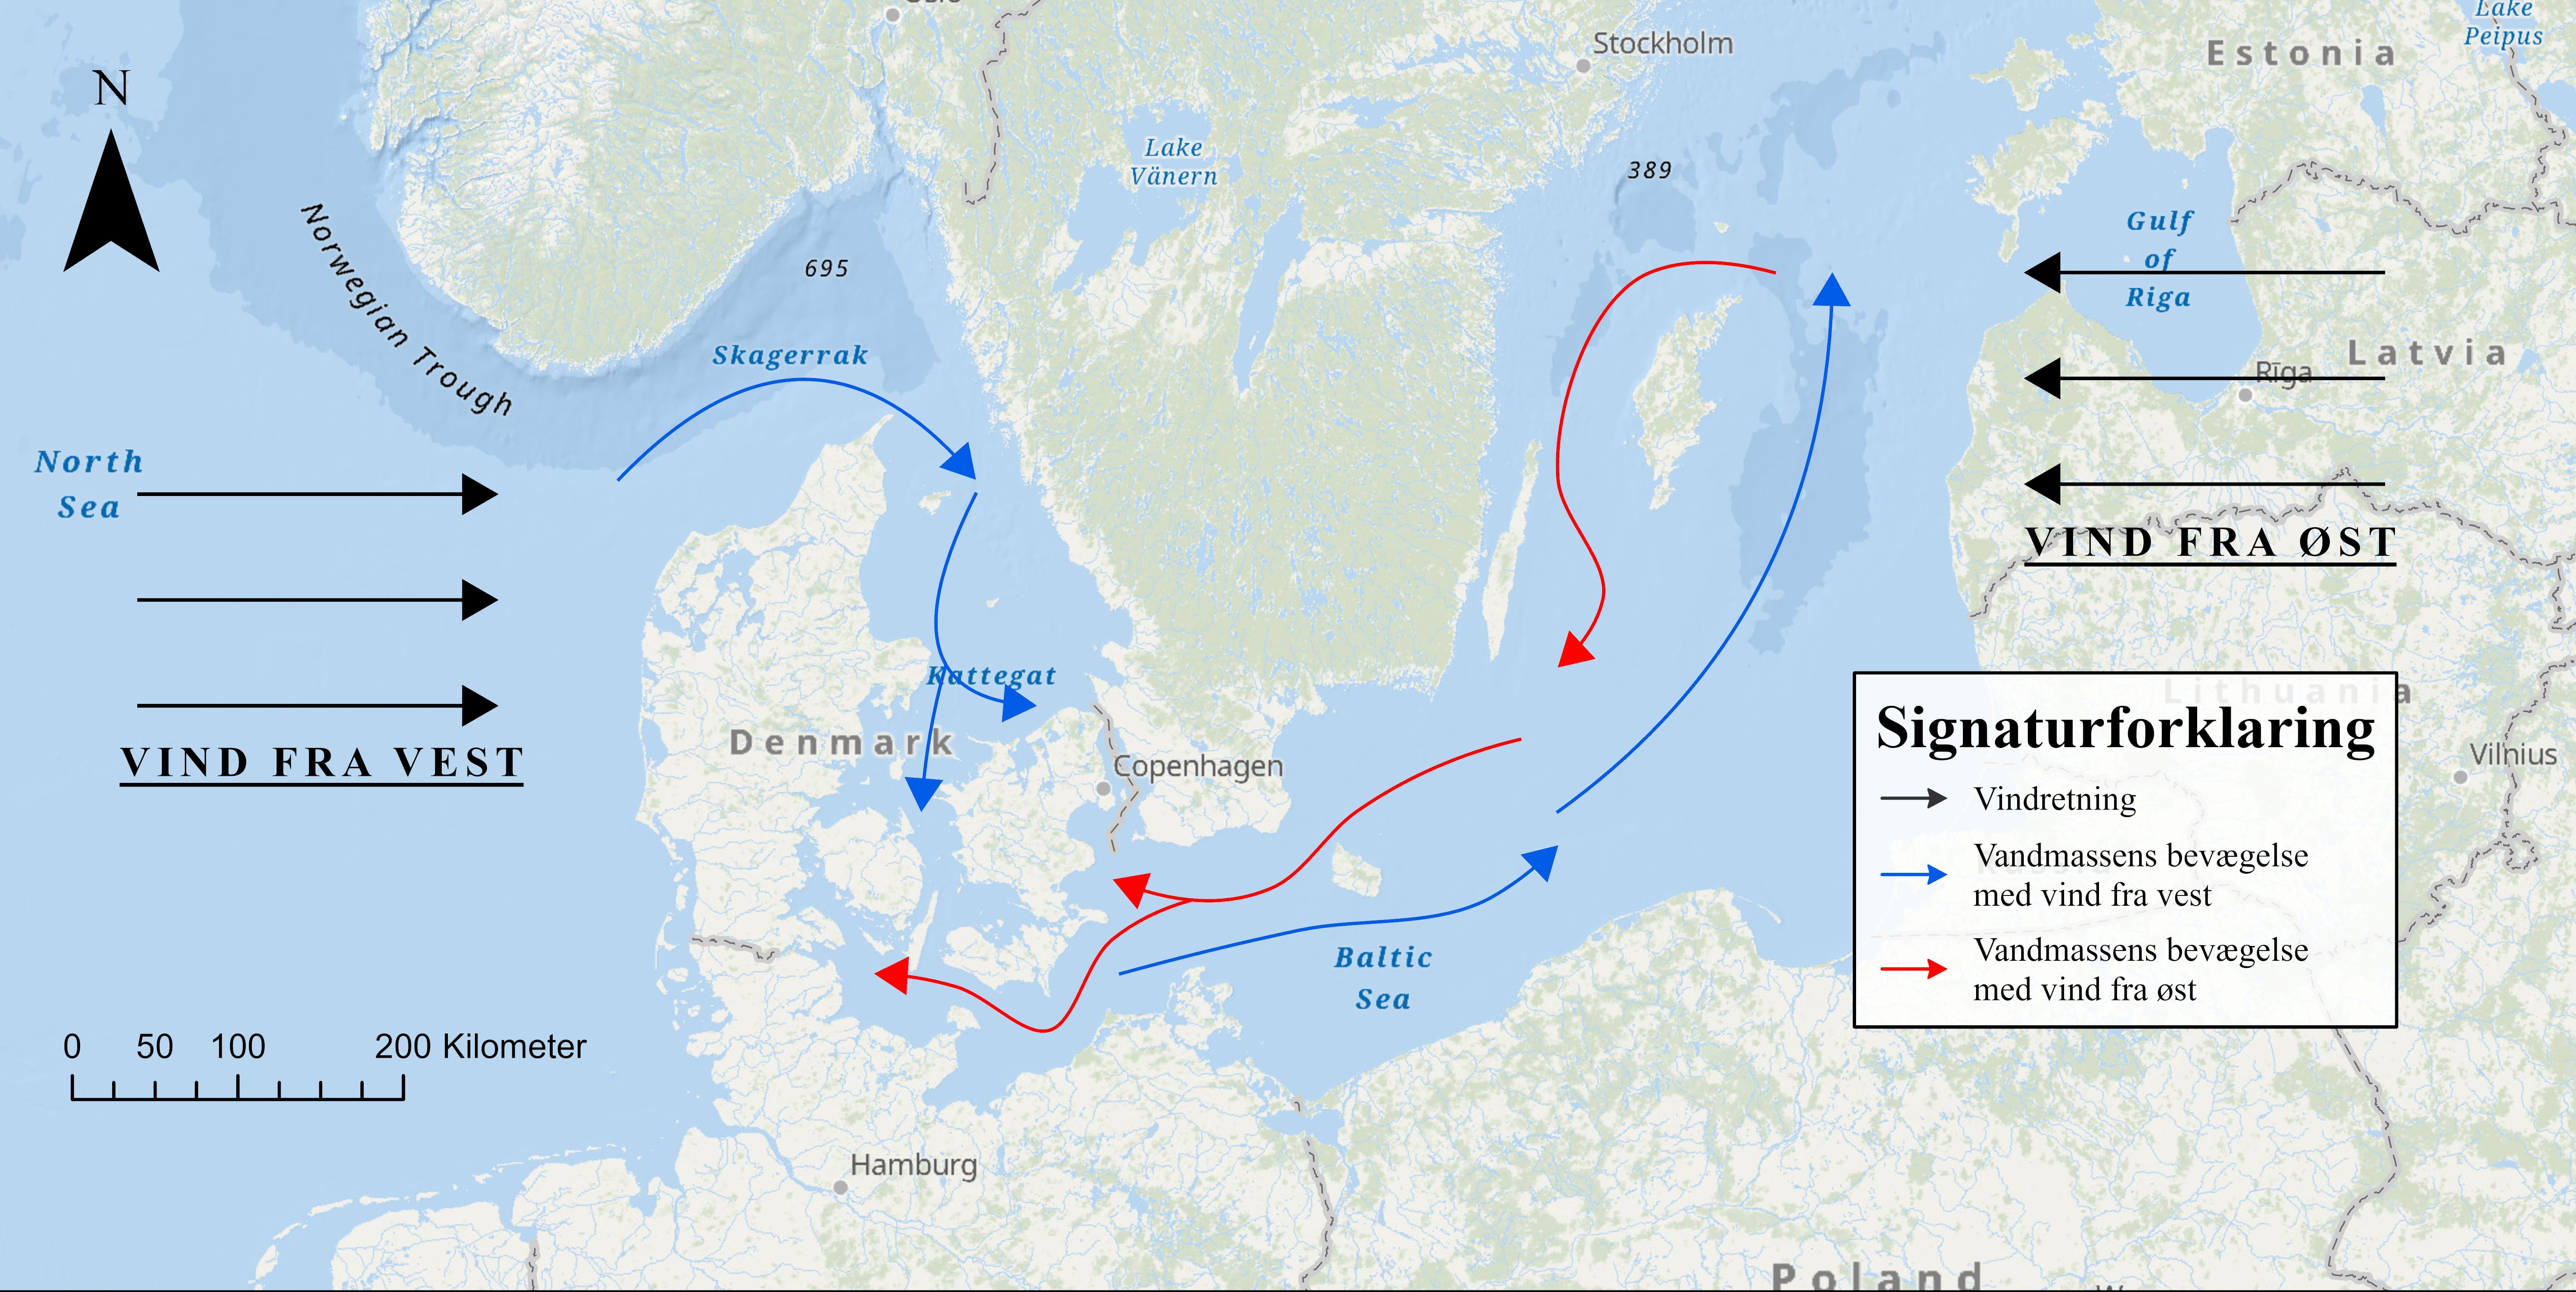
\includegraphics[width=0.8\linewidth]{images/teori/bathtub effect graphics.jpg}
    \caption{Illustration af badekarseffekten i Østersøen. De sorte pile indikerer vindretning og de blå og røde pile indikerer bevægelsen af vandmassen ved henholdsvis vest- og østenvind. Kilde: Egen illustration, baggrundskort fra Esri}
    \label{Figur: Bathtub effect}
\end{figure}

Historisk har flere betydelige stormfloder i Danmark, såsom stormfloderne i november 1872, november 2006 and oktober 2023, været forårsaget af en kombination af længerevarende vestenvind efterfulgt af østenvind og den resulterende badekarseffekt \citep{kystdirektoratet_stormfloder}.

\subsection{Stormfloden den 20 oktober 2023} \label{Afsnit: Stormfloden den 20 oktober 2023}
I første halvdel af oktober 2023 blev der observeret moderate vindforhold med gennemsnitlig middelvind på 5,5 m/s og en gennemsnitlig maksimal 10.min middelvind på 18,3 m/s fra vest, hvilket medførte en betydelig vandtransport gennem Kattegat og videre ind i Østersøen \citep{dmi_vejrarkiv}. \\

Onsdag den 18. oktober skiftede vindretningen til øst (figur \ref{Figur: Vinddata Danmark}) forårsaget af trykforskelle mellem et højtryksystem over det nordlige Skandinavien og et lavtrykssystem vest for Storbritannien \citep{kiesel_brief_2024}, og middelvindhastigheden steg i hele landet til 12,2 m/s og maksimale 10.min middelvind til 28,3 m/s om aftenen den 20. oktober 2023. Derudover faldt lufttrykket i Danmark til omkring 995 hPa, målt maksimale vindstød på ca. 34 m/s og er derfor klassificeret som orkanstyrke \citep{dmi_vejrarkiv}. 
\begin{figure} [H]
    \centering
    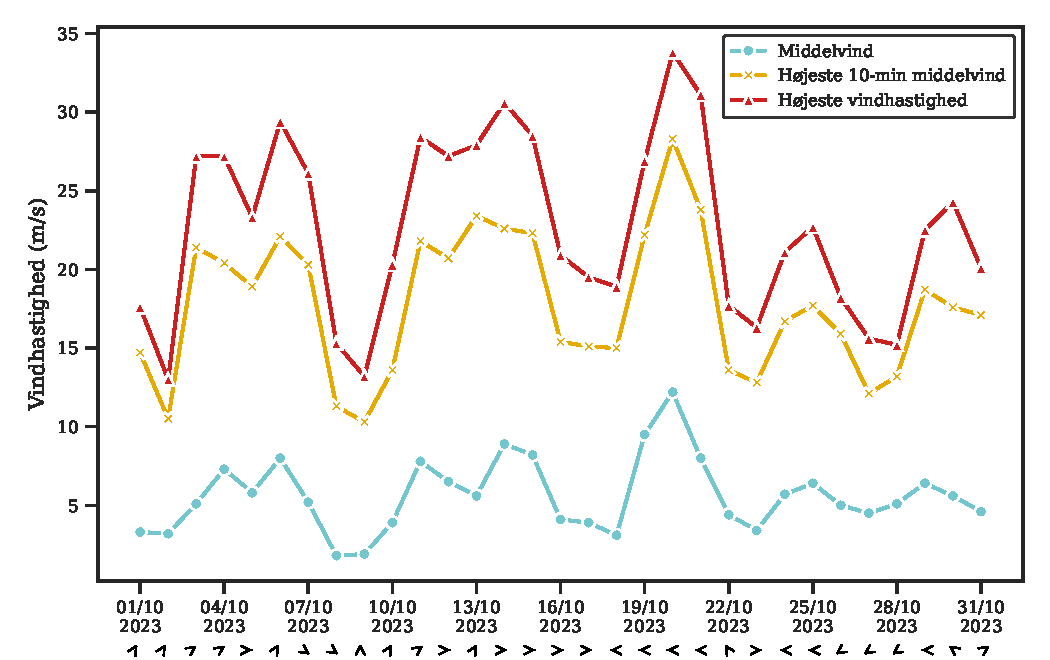
\includegraphics[width=0.9\linewidth]{images/teori/vinddata_grafer/Danmark_vinddata.pdf}
    \caption{Vinddata for Danmark i oktober 2023 der viser middelvind, højeste 10.min middelvind og højeste vindhastighed i m/s. De sorte pile i bunden indikerer hvilken retning vinder blæser imod. Kilde: Data fra \cite{dmi_vejrarkiv} }
    \label{Figur: Vinddata Danmark}
\end{figure}

Kombinationen af kraftig vind fra øst og stor vandtransport ind i Østersøen over en periode på 15 dage resulterede ifølge \cite{kystdirektoratet_stormflod2023} i markante vandstandsstigninger i de indre farvande af Syddanmark i løbet af eftermiddagen den 20. oktober. Den højeste officielle vandstand målt under stormfloden blev målt i Aabenraa Havn på 2,16 m over dagligt vande \citep{damberg_vaerste_2023}. Disse forhold forårsagede omfattende skader af sommerhusområder, kystnære områder, havne og byer \citep{kystdirektoratet_stormflod2023, naturskaderadet_anmeldelser_2023}. \\
Stormfloden der ramte Danmark, påvirkede også en række af landets naboer. Nordtyskland og den sydlige del af Sverige observerede forhøjet vandstand og kraftig vind \citep{kiesel_brief_2024}. Samtidig blev der observeret en orkan over Storbritannien der resulterede i ekstrem nedbør over de Britiske Øer \citep{met_office_storm_2023}.  




